\documentclass{Preport}

\usepackage{hyperref}
\hypersetup{
    colorlinks=true,
}

\usepackage{float}
\usepackage{amsmath}
\usepackage[european]{circuitikz}

\setlength{\intextsep}{4pt}
\setlength{\abovecaptionskip}{4pt}
\setlength{\belowcaptionskip}{0pt}

\exname{交流电路功率因数实验} %实验名称
\instructor{杨佳楠} %指导教师
\class{电科2502} %班级
\name{管云哲} %姓名
\stuid{3250104519} %学号

\nyear{2026} %年
\nmonth{11} %月
\nday{3} %日
\nweekday{二} %星期几

\begin{document}
\setcounter{page}{1}
\makecover

\section{预习报告（10分）}
\subsection{实验综述（5分）}
（自述实验现象、实验原理和实验方法，包括必要的光路图、电路图、公式等。不超过500字。）

实验现象：闭合开关，启辉器放电使灯丝预热；启辉器随后断开，镇流器产生高压脉冲点亮灯管，之后镇流器起限流作用。并联电容后，总电流随电容增大先减小后增大。

实验原理：交流电路的平均功率为 $P=UI\cos\varphi$，其中 $\cos\varphi=P/(UI)$ 称为功率因数。日光灯是电感性负载，可等效为灯管电阻 $R$ 与镇流器电感 $L$、内阻 $r$ 串联。灯管电流 $I_L$ 滞后总电压 $U$ 相位角 $\varphi$，故 $\cos\varphi<1$。在负载两端并联电容 $C$ 后，电容电流 $I_C$ 超前 $U$ 相位 $90^\circ$，总电流 $I=I_L+I_C$。若 $C$ 取值合适，总电流减小，相位差 $\varphi'<\varphi$，功率因数提高；$C$ 过大时总电流转为容性，$\cos\varphi$ 反而下降。

\begin{figure}[H]
    \centering
    \begin{minipage}[b]{0.62\linewidth}
        \centering
        \begin{circuitikz}[european, scale=0.72, transform shape]
            % 电源
            \draw (0,0) to[sV, l=$U$] (0,3.2);
            % 电压表
            \draw (0,3.2) -- (1.4,3.2) to[rmeter, t=$V$] (1.4,0) -- (0,0);
            % 功率表与电流表
            \draw (1.4,3.2) -- (2.4,3.2)
                  to[rmeter, t=$W$] (3.9,3.2)
                  to[rmeter, t=$A$] (5.4,3.2)
                  -- (6.4,3.2);
            % 并联电容支路
            \draw (6.4,3.2) to[vC, l=$C$] (6.4,0);
            % 镇流器
            \draw (6.4,3.2) -- (7.2,3.2) to[american inductor, l=$M$] (8.6,3.2) -- (9.4,3.2);
            % 灯管
            \draw (9.4,3.2) to[lamp, l_=$L$] (9.4,0.8) -- (9.4,0);
            % 启辉器
            \draw (9.4,3.2) -- (11,3.2)
                  to[lamp, l=$S$] (11,0.8)
                  -- (9.4,0.8);
            % 返回总线
            \draw (11,0.8) -- (11,0) -- (0,0);
            \node[circ] at (6.4,3.2) {};
            \node[circ] at (9.4,3.2) {};
            \node[circ] at (9.4,0.8) {};
        \end{circuitikz}\\[-1mm]
        {\small (a) 实验电路}
    \end{minipage}\hfill
    \begin{minipage}[b]{0.34\linewidth}
        \centering
        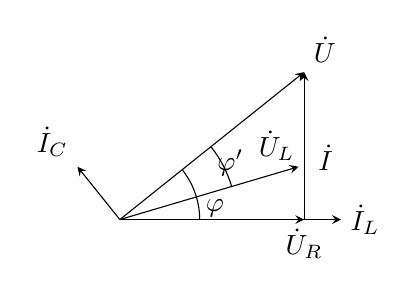
\begin{tikzpicture}[scale=0.78, >=stealth]
            \draw[->] (0,0) -- (3.6,0) node[right] {$\dot I_L$};
            \draw[->] (0,0) -- (3.0,2.4) node[above right] {$\dot U$};
            \draw[->] (0,0) -- (3.0,0) node[below] {$\dot U_R$};
            \draw[->] (3.0,0) -- (3.0,2.4) node[midway, left] {$\dot U_L$};
            \draw[->] (0,0) -- (-0.69,0.86) node[above left] {$\dot I_C$};
            \draw[->] (0,0) -- (2.91,0.86);
            \node at (3.35,1.0) {$\dot I$};
            \draw (1.3,0) arc (0:38.7:1.3);
            \node at (1.55,0.18) {$\varphi$};
            \draw (1.82,0.54) arc (16.5:38.7:1.9);
            \node at (1.80,0.92) {$\varphi'$};
        \end{tikzpicture}\\[-1mm]
        {\small (b) 相量图}
    \end{minipage}
    \caption{交流电路功率因数实验电路与并联电容前后的相量图}
    \label{fig:principle}
\end{figure}

实验方法：用电压表、电流表、功率表测额定电压下日光灯电路的 $U$、$I$、$P$，由 $\cos\varphi=P/(UI)$ 计算功率因数。将电容从 $1\,\mu\mathrm{F}$ 逐级增至 $7\,\mu\mathrm{F}$，计算各组的 $\cos\varphi$ 并作 $\cos\varphi$--$C$ 散点图，找出使 $\cos\varphi$ 最大的电容值。

\subsection{实验重点（3分）}
（简述本实验的学习重点，不超过100字。）

理解功率因数的物理意义及电感性负载 $\cos\varphi<1$ 的原因；掌握并联电容提高功率因数的方法；熟悉日光灯电路的结构与启辉、限流过程；学会用电压表、电流表、功率表测量并计算 $\cos\varphi$，由 $\cos\varphi$--$C$ 曲线确定最佳电容。

\subsection{实验难点（2分）}
（简述本实验的实现难点，不超过100字。）

日光灯启辉过程涉及启辉器与镇流器的配合，原理较抽象；电容需逐级接入，避免过大使总电流回升、功率因数下降。

{\fangsong 注意事项：
\begin{enumerate}[label=\arabic*.]
    \item 用PDF格式上传“实验报告”，文件名：学生姓名+学号+实验名称+周次。
    \item “实验报告”必须递交在“学在浙大”本课程内对应实验项目的“作业”模块内。
    \item “实验报告”成绩必须在“浙江大学物理实验教学中心网站”-“选课系统”内查询。
    \item 教学评价必须在“浙江大学物理实验教学中心网站”-“选课系统”内进行，学生必须进行教学评价，才能看到实验报告成绩，教学评价须在本次实验结束后3天内进行。
\end{enumerate}}
\begin{center}
    \fbfangsong{浙江大学物理实验教学中心制}
\end{center}
\end{document}
